\chapter{Related Work}
\label{chapter:relatedwork}

\section{Opinion spam}\label{section:opinion-spam}

The opinion spam problem was first formulated by Jindal and Liu in the context of product reviews, \citet{Jindal2008}. By analyzing several million reviews from the popular Amazon.com, they showed how widespread the problem of fake reviews was. The existing detection methods can be split in the context of machine learning into supervised and unsupervised approaches. Second, they can be split into three categories by their features: behavioral, linguistic or those using a combination of these two.
They categorized spam reviews into three categories: non-reviews, brand-only reviews and untruthful reviews. The authors ran a logistic regression classifier on a model trained on duplicate or near-duplicate reviews as positive training data, i.e. fake reviews, and the rest of the reviews they used as truthful reviews. They combined reviewer behavioral features with textual features and they aimed to demonstrate that the model could be generalized to detect non-duplicate review spam. This was the first documented research on the problem of opinion spam and thus did not benefit from existing training databases. The authors had to build their own dataset, and the simplest approach was to use near-duplicate reviews as examples of deceptive reviews. Although this initial model showed good results, it is still an early investigation into this problem.

\citet{Lim2010} is also an early work on detecting review spammers which proposed scoring techniques for the spamicity degree of each reviewer. The authors tested their model on Amazon reviews, which were initially taken through several data preprocessing steps. In this stage, they decided to only keep reviews from highly active users - users that had written at least 3 reviews. The detection methods are based on several predefined abnormalities indicators, such as general rating deviation, early deviation - i.e. how soon after a product appears on the website does a suspicious user post a review about it or very high/low ratings clusters. The features weights were linearly combined towards a spamicity formula and computed empirically in order to maximize the value of the normalized discounted cumulative gain measure. The measure showed how well a particular ranking improves on the overall goal. The training data was constructed as mentioned earlier from Amazon reviews, which were manually labeled by human evaluators. Although an agreement measure is used to compute the inter-evaluator agreement percentage, so that a review is considered fake if all of the human evaluators agree, this method of manually labeling deceptive reviews has been proven to lead to low accuracy when testing on real-life fake review data. 
First, \citet{Ott2011} demonstrated that it is impossible for humans to detect fake reviews simply by reading the text. Second, \citet{Mukherjee2012} proved that not even fake reviews produced through crowdsourcing methods are valid training data because the models do not generalize well on real-life test data.

\citet{Wang2012} considered the triangular relationship among stores, reviewers and their reviews. This was the first study to capture such relationships between these concepts and study their implications. They introduced 3 measures meant to do this: the stores’ reliability, the trustworthiness of the reviewers and the honesty of the reviews. Each concept depends on the other two, in a circular way, i.e. a store is more reliable when it contains honest reviews written by trustworthy reviewers and so on for the other two concepts. They proposed a heterogeneous graph based model, called the review graph, with 3 types of nodes, each type of node being characterized by a spamicity score inferred using the other 2 types. In this way, they aimed to capture much more information about stores, reviews and reviewers than just focus on behavioral reviewer centric features. This is also the first study on store reviews, which are different than product reviews. The authors argue that when looking at product reviews, while it may be suspicious to have multiple reviews from the same person for similar products, it is ok for the same person to buy multiple similar products from the same store and write a review every time about the experience. In almost all fake product reviews, studies which use the cosine similarity as a measure of review content alikeness, a high value is considered as a clear signal of cheating, since the spammers do not spend much time writing new reviews all the time, but reuse the exact same words. However, when considering store reviews, it is possible for the same user to make valid purchases from similar stores, thus reusing the content of his older reviews and not writing completely different reviews all the time. \citet{Wang2012} used an iterative algorithm to rank the stores, reviewers and reviews respectively, claiming that top rankers in each of the 3 categories are suspicious. They evaluated their top 10 top and bottom ranked spammer reviewers results using human evaluators and computed the inter-evaluator agreement. The evaluation of the resulted store reliability score, again for the top 10 top and bottom ranked stores was done by comparison with store data from Better Business Bureaus, a corporation that keeps track businesses reliability and possible consumer scams. 

\citet{Xie2012} observed that the vast majority of reviewers (more than 90\% in their study or resellerratings.com reviews up to 2010) only wrote one review, so they have focused their research on this type of reviewers. They also claim, similarly to \citet{Feng2012}, that a flow of fake reviews coming from a hired spammer distorts the usual distribution of ratings for the product, leaving distributional traces behind. Xie et al. observed the normal flow of reviews is not correlated with the given ratings over time. Fake reviews come in bursts of either very high ratings, i.e. 5-stars, or very low ratings, i.e. 1-star, so the authors aim to detect time windows in which these abnormally correlated patterns appear. They considered the number of reviews, average ratings and the ratio of singleton reviews which stick out when looking over different time windows. The paper makes important contributions to opinion spam detection by being the first study to date to formulate the singleton spam review problem. Previous works have disregarded this aspect completely by purging singleton reviews from their training datasets and focusing more on tracking the activity of reviewers as they make multiple reviews. It is of course reasonable to claim that the more information is saved about a user and the more data points about a user's activity exist, the easier it is to profile that user and assert with greater accuracy whether he is a spammer or not. Still, it is simply not negligible that a large percentage of users on review platforms write only one review.  

\citet{Feng2012} published the first study to tackle the opinion spam as a distributional anomaly problem, considering crawled data from Amazon and TripAdvisor. They claim product reviews are characterized by natural distributions which are distorted by hired spammers when writing fake reviews. Their contribution consists of first introducing the notion of natural distribution of opinions and second of conducting a range of experiments that finds a connection between distributional anomalies and the time windows when deceptive reviews were written. For the purpose of evaluation they used a gold standard dataset containing 400  known deceptive reviews written by hired people, created by \citet{Ott2011}. Their proposed method achieves a maximum accuracy of only 72.5\% on the test dataset and thus is suitable as a technique to pinpoint suspicious activity within a time window and draw attention on suspicious products or brands. This technique does not solely represent however a complete solution where individual reviews can be deemed as fake or truthful, but simply brings to the foreground delimited short time windows where methods from other studies can be applied to detect spammers.

\citet{Li2011} have used supervised learning and manually labeled reviews crawled from Epinions to detect product review spam. They also added to the model the helpfulness scores and comments the users associated with each review. Due to the dataset size of about 60K reviews and the fact that manual labeling was required, an important assumption was made - reviews that receive fewer helpful votes from people are more suspicious. Based on this assumption, they have filtered out review data accordingly, e.g. only considering reviews which have at least 5 helpfulness votes or comments.
They achieved a 0.58 F-Score result using their supervised method model, which outperformed the heuristic methods used at that time to detect review spam. However, this result is very low when compared with that of more recent review spam detection models. The main reason for this has been the training of the model on manually labeled fake reviews data, as well as the initial data pre-processing step where reviews were selected based on their helpfulness votes. \citet{Mukherjee2013} also makes the  assumption that deceptive reviews get less votes. But their model evaluation later showed that helpfulness votes not only perform poorly but they may also be abused - groups of spammers working together to promote certain products may give many votes to each others reviews. The same conclusion has been also expressed by \citet{Lim2010}.

\citet{Ott2011} produced the first dataset of gold-standard deceptive opinion spam, employing crowdsourcing through the Amazon Mechanical Turk. They demonstrated that humans cannot distinguish fake reviews by simply reading the text, the results of these experiments showing an  at-chance probability. The authors found that although part-of-speech n-gram features give a fairly good prediction on whether an individual review is fake, the classifier actually performed slightly better when psycholinguistic features were added to the model. The expectation was also that truthful reviews resemble more of an informative writing style, while deceptive reviews are more similar in genre to imaginative writing. The authors coupled the part-of-speech tags in the review text which had the highest frequency distribution with the results obtained from a text analysis tool previously used to analyze deception. Testing their classifier against the gold-standard dataset, they revealed clue words deemed as signs of deceptive writing. However, this can be seen as overly simplistic, as some of these words, which according to the results have a higher probability to appear in a fake review, such as "vacation" or "family", may as well appear in truthful reviews. The authors finally concluded that the domain context has an important role in the feature selection process. Simply put, the imagination of spammers is limited - e.g. in the case of hotel reviews, they tend to not be able to give spatial details regarding their stay. While the classifier scored good results on the gold-standard dataset, once the spammers learn about them, they could simply avoid using the particular clue words, thus lowering the classifier accuracy when applied to real-life data on the long term. 

\citet{Mukherjee2012} were the first to try to solve the problem of opinion spam resulted from a group collaboration between multiple spammers. The method they proposed first extracts candidate groups of users using a frequent itemset mining technique. For each group, several individual and group behavioral indicators are computed, e.g. the time differences between group members when posting, the rating deviation between group members compared with the rest of the product reviewers, the number of products the group members worked together on, or review content similarities. The authors also built a dataset of fake reviews, with the help of human judges which manually labeled a number of reviews. They experimented both with learning to rank methods, i.e. ranking of groups based on their spamicity score and with classification using SVM and logistic regression, using the labeled review data for training. The algorithm, called GSRank considerably outperformed existing methods by achieving an area under the curve result (AUC) of 95\%. This score makes it a very strong candidate for production environments where the community of users is very active and each user writes more than one review. However, not many users write a lot of reviews, there exists a relatively small percentage of "elite" contributing users. So this method would best be coupled with a method for detecting singleton reviewers, such as the method from \citet{Xie2012}. 

\citet{Mukherjee2013b} have questioned the validity of previous research results based on supervised learning techniques trained on Amazon Mechanical Turk (AMT) generated fake reviews. They tested the method of \citet{Ott2011} on known fake reviews from Yelp. The assumption was that the company had perfected its detection algorithm for the past decade and so its results should be trustworthy. Surprisingly, unlike \citet{Ott2011} which reported a 90\% accuracy using the fake reviews generated through the AMT tool, \citet{Mukherjee2013b} experiments showed only a 68\% accuracy when they tested Ott's model on Yelp data. This led the authors to claim that any previous model trained using reviews collected through the AMT tool can only offer near chance accuracy and is useless when applied on real-life data. However, the authors do not rule out the effectiveness of using n-gram features in the model and they proved the largest accuracy obtained on Yelp data was achieved using a combination of behavioral and linguistic features. Their experiments show little improvement over accuracy when adding n-gram features. Probably the most interesting conclusion is that behavioral features considerably outperform n-gram features alone. 

\citet{Mukherjee2013} built an unsupervised model called the Author Spamicity Model that aims to split the users into two clusters - truthful users and spammers. The intuition is that the two types of users are naturally separable due to the behavioral footprints left behind when writing reviews. The authors studied the distributional divergence between the two types and tested their model on real-life Amazon reviews. Most of the behavioral features in the model have been previously used in two previous studies by \citet{Mukherjee2012} and \citet{Mukherjee2013b}. In these studies though, the model was trained using supervised learning. The novelty about the proposed method in this paper is a posterior density analysis of each of the features used. This analysis is meant to validate the relevance of each model feature and also increase the knowledge on their expected values for truthful and fake reviews respectively.

\citet{Fei2013} focused on detecting spammers that write reviews in short bursts. They represented the reviewers and the relationships between them in a graph and used a graph propagation method to classify reviewers as spammers. Classification was done using supervised learning, by employing human evaluation of the identified honest/deceptive reviewers. The authors relied on behavioral features to detect periods in time when review bursts per product coincided with reviewer burst, i.e. a reviewer is very prolific just as when a number of reviews which is higher than the usual average of reviews for a particular product is recorded. The authors discarded singleton reviewers from the initial dataset, since these provide little behavior information - all the model features used in the burst detection model require extensive reviewing history for each user. By discarding singleton reviewers, this method is similar to the one proposed by \citet{Mukherjee2012}. These methods can thus only detect fake reviews written by elite users on a review platform. Exploiting review posting bursts is an intuitive way to obtain smaller time windows where suspicious activity occurs. This can be seen as a way to break the fake review detection method into smaller chunks and employ other methods which have to work with considerably less data points. This would decrease the computational and time complexity of the detection algorithm. 

\citet{Mukherjee2013a} made an interesting observation in their study: the spammers caught by Yelp's filter seem to have "overdone faking" in their try to sound more genuine. In their deceptive reviews, they tried to use words that appear in genuine reviews almost equally frequently, thus avoiding to reuse the exact same words in their reviews. This is exactly the reason why a cosine similarity measure is not enough to catch subtle spammers in real life scenarios, such as Yelp's. 

\clearpage

\section{Textual similarity}\label{section:textual-similarity}

Textual similarity is ubiquitous in most natural language processing problems, such as text classification, text summarization, word-sense disambiguation, machine translation and information retrieval. Computing the similarity of text documents boils down to computing the similarity of their words. Any two words can be considered similar if some relation can be defined between them. This relation can be of synonymy/antonymy, i.e. they refer to the same/opposite thing. Or they might be used in the same context, e.g. political - party, legislation and parliament are similar in this context. Or they are related through a hierarchy, e.g. liquid, beer and pilsner. Or they could simply be the same part-of-speech words, as in both are nouns or verbs for example.

\subsection{Vectorial-based measures}\label{section:vectorial-based-measures}

The vector space model is widely used in information retrieval to find the best matching set of relevant documents for an input query. Given two documents, each of them can be modeled as a n-dimensional vector where each of the dimensions is one of its words. The goal of finding the similarity between the two documents is translated now into a vector algebra problem, where the goal is to compute the distance between their two word-vectors, by measuring the cosine angle between them. \citet{Salton1971} experimented with lexical matching using the cosine correlation and reported good results in the SMART Information Retrieval System, \citet{SMART}.

For two vectors $T_1$ and $T_2$, their cosine similarity can be formulated as
\begin{equation}
\cos ({ T_1},{ T_2})= {{T_1} {T_2} \over \|{ T_1}\| \|{ T_2}\|} = \frac{ \sum_{i=1}^{n}{{ T_1}_i{ T_2}_i} }{ \sqrt{\sum_{i=1}^{n}{({ T_1}_i)^2}} \sqrt{\sum_{i=1}^{n}{({ T_2}_i)^2}} }
\end{equation}

The vector based model has the major advantages of being simple to implement, allowing partial matching and providing very good runtime performance, but a simple model has also its fair share of disadvantages. It assumes the query words are statistically independent, although this is usually not the case. If all words in a document would be orthogonal or independent of each other, the document would not make any sense. Furthermore, it captures no semantic relationships, so that documents from the same context but with words from different vocabularies are not associated. Various improvements to this model, such as stopwords removal, part-of-speech tagging or giving different weights to certain words in the documents  have been proposed over time, \citet{Salton1988}.

Although these additions have increased the relevance of the results, they cannot capture any semantic relations inside the documents. Still, even with these obvious disadvantages, the vectorial model is widely used in production systems because of its simplicity and runtime performance. 

\subsection{Knowledge-based measures}\label{section:knowledge-based-measures}

According to \citet{Budanitsky1999}, there are a few notable approaches to measure semantic relatedness. The earliest approach is not surprisingly the dictionary-based method, which tried to link each word with the words in its dictionary definition. This would lead to a word network where high density areas would represent more closely related words. The thesaurus-based approach followed and grouping words and phrases into concepts meant a lot of manual work. Algorithms built on top of this thesaurus would only be able to return a boolean result of whether two concepts were related or not, without being able to compute any semantic distance inside the network. Finally, lexical databases such as WordNet made it easier for concepts to be linked and form a navigable semantic network. 

WordNet is one of the largest lexical databases for the English language, comprising of nouns, verbs, adjectives and adverbs grouped in synonymical rings, i.e. groups of words, which in the context of information retrieval applications are considered semantically equivalent. These groups are then connected through relations into a larger network which can be navigated and used in computational linguistics problems, \citet{WordNet}. 
The hierarchical relations capture different abstractions:
\begin{itemize}
\item hyponymy - super-subordinate or a \textit{is-a} relation. An example is that of \textit{furniture-bed-bunkbed}: \textit{bed} is part of the \textit{furniture} category and \textit{bunkbed} is a smaller type of \textit{bed}.
\item meronymy - part-whole relation: \textit{computer-keyboard} or \textit{electronic device-battery}. This kind of relation can be inferred in sub-parts of the superordinates, so that a \textit{laptop}, which is a subordinate of \textit{computer} will also be closely connected to \textit{keyboard}.
\item verbs are also organized in a top-bottom hierarchy, corresponding to their specificity. At the top there are the more abstract words, such as \textit{discussion}, then at the next level there is \textit{talk} and further down comes \textit{whisper}.
\end{itemize}
 
\begin{figure}[ht!]
\centering
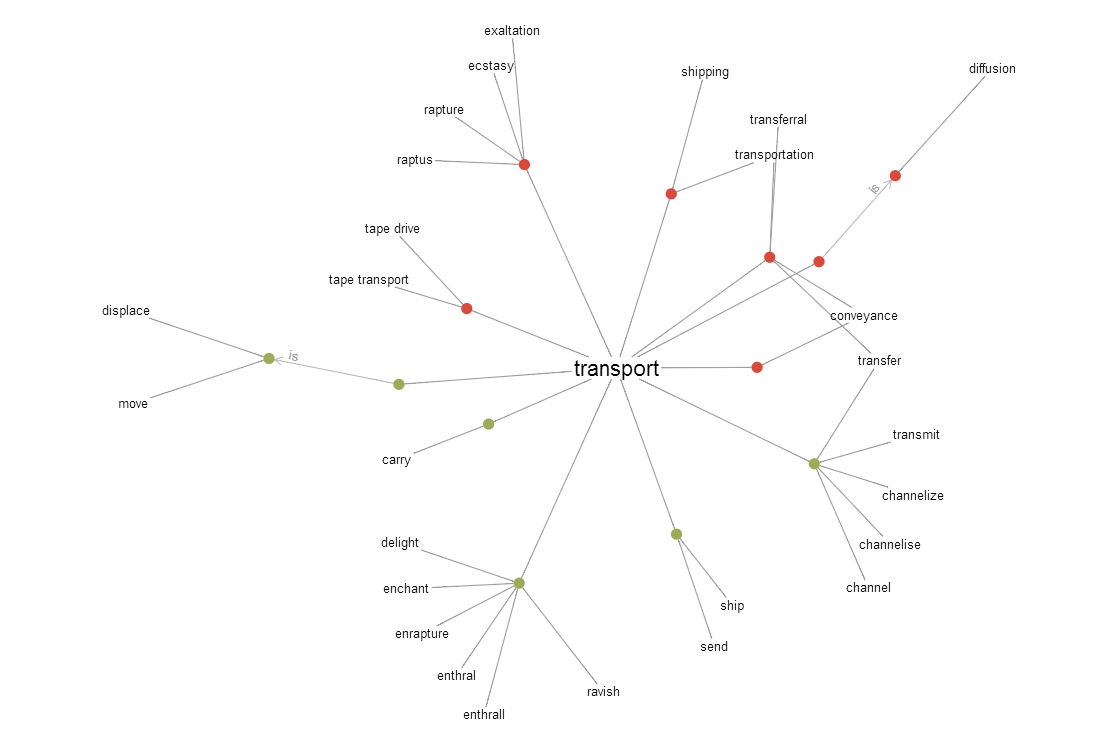
\includegraphics[width=\textwidth]{figures/transport.png}
\caption{An example of the WordNet structure for the word \textit{transport}}
\label{transport}
\end{figure} 

\citet{Mihalcea2006} proposed a method to extend the word-to-word similarity inside WordNet to the document level and proved their method outperformed the existing vectorial approaches. They combined the maximum value from six well known word-to-word similarity measures based on distances in WordNet - Leacock \& Chodorow, Lesk, Wu \& Palmer, Resnik, Lin, Jiang \& Conrath - with the inverse document frequency specificity metric \textit{idf}. \textit{Idf} is defined by the logarithm of the number of documents inside the corpus divided by the number of documents containing the specific word. 

For the purpose of this project, I have only considered Mihalcea’s measure, because it was proven to outperform any of the six word-to-word semantic measures taken individually. Equation \ref{eq:mihalcea-definition} formulates the semantic similarity between two texts $T_1$ and $T_2$.

\begin{equation}\label{eq:mihalcea-definition}
sim ({ T_1},{ T_2})= \frac{1}{2}(\frac{\sum\limits_{w\in\{T_1\}}{(maxSim(w,T_2)*idf(w))}}{\sum\limits_{w\in\{T_1\}}{idf(w)}} + \frac{\sum\limits_{w\in\{T_2\}}{(maxSim(w,T_1)*idf(w))}}{\sum\limits_{w\in\{T_2\}}{idf(w)}})
\end{equation}

The similarity score is a real number in [0, 1], 1 being associated with identical texts. Mihalcea’s approach takes into account nouns, verbs, adjectives and adverbs and computes the similarity between the same part-of-speech words, i.e. nouns against nouns and verbs against verbs. It uses simple lexical matching for adjectives and adverbs. 

Consider the following short fake reviews and suppose the two texts would be regarded as suspicious only when the similarity score would exceed a threshold of 0.5. 

\begin{description}
\item[$T_1$]: \textit{I have to say that this was one of the fastest loan companies I have ever dealt with! They took the time to explain everything and went out of their way to ensure my satisfaction. I will definitely use them again.}
\item[$T_2$]: \textit{I swear, it's like this company runs on energy drinks or something! It's the fastest loan I've ever applied to and been approved for. This is the most awesome company I've worked with, financially speaking. I'd recommend them to anybody, for anything!}
\end{description}

The cosine similarity gives a score of 0.24, thus is would not get flagged as highly similar, while Mihalcea’s semantic measure outputs a similarity of 0.66, outperforming the vectorial model.

\clearpage

\section{Aspect-based opinion mining}\label{section:aspect-based-opinion-mining}

Aspect mining is a new opinion mining technique used to extract product attributes, also called aspects from reviews. Aspects are things like \textit{screen}, \textit{battery} or \textit{camera}. People use different words to describe the same aspect - \textit{laptop}, \textit{notebook}, \textit{notebook computer}. These aspects are usually followed by words expressing people's sentiments about them, such as \textit{small screen} or \textit{low-quality camera}. So reviews can be simplistically abstracted as a set of aspect-sentiment pairs, linked together by stopwords.

It is becoming increasingly difficult to handle the large number of opinions posted on review platforms and at the same time offer this information in a useful way to each user so he or she can make a decision fast whether to buy the product or not. Aspect-based aggregations and short review summaries are used to group and condense what other users think about the product in order to personalize the content served to a new user and shorten the time he needs to make a buying decision.

The techniques used to extract aspects from reviews have been classified by \citet{BingLiu2012} into frequency-based approaches and model-based approaches. The first technique relies on finding frequent nouns to identify aspects. This has been proven to be very effective and easy to implement in production systems. The downside is that it requires manual tuning and it misses infrequent aspects, which might contain useful information. The model-based approaches can be divided in two subcategories: 
\begin{itemize}
\item supervised learning models - where a labeled dataset of aspects is available upfront.
\item unsupervised topic models - no labeled dataset is required upfront, the model learns the underlying topics which make up a document. A topic is made up of several semantically linked aspects or can be a viewed as an aspect in itself.
\end{itemize}

The supervised learning models overcome the disadvantages of the frequency-based methods and avoid cumbersome tuning because they work on labeled data. Their main disadvantage is obvious, they need the labeled data upfront.

Topic models are statistical models where each document is seen as a mixture of latent topics, each of the topics contributing with certain proportions to the document. Formally, a topic is defined as a distribution over a fixed vocabulary of words as explained more thoroughly in \citet{Blei2012}. These models have received increasing attention in recent years since they do not require manually labeled data to work, although they perform best when trained on large document corpuses. 

There are two main topic models, with many variations deriving from them:
\begin{itemize}
\item Probabilistic Latent Semantic Indexing (PLSI) - technique for the analysis of words co-occurrence in document corpuses
\item Latent Dirichlet Allocation (LDA) - statistical model used to capture the intuition that documents are mixtures of latent topics
\end{itemize}

Reviews are in fact short documents, so they can be abstracted as a mixture of latent topics. The topics can be considered equivalent to the review aspects and thus the problem of extracting aspects can be translated to a topic modeling problem. As \citet{Moghaddam2013} notes, the topics may refer to both aspects - \textit{laptop}, \textit{screen} and sentiments - \textit{expensive}, \textit{broken}. Several LDA-based models have been proposed by \citet{Moghaddam:2012:DLM:2396761.2396863} which also evaluated which technique among frequent nouns, POS patterns and opinion phrases (<aspect,sentiment> pairs) performs best.

Extending this logic, it should be possible to apply topic modeling to the problem of detecting opinion spam, by comparing the similarity between the extracted aspects in the reviews with a fixed spam threshold. One large advantage when applying this technique is the model would be language agnostic, meaning it could infer semantics in reviews regardless of the language. This is not implicit when using WordNet and although WordNets have been created for other languages besides English, such as \citet{EuroWordNet}, none match the scale of the English corpus.

As mentioned before, the imagination of a spammer is limited and thus he will not be able to write completely different reviews about an imaginary experience every time. The hypothesis to test is if spammers are reusing the same aspects between reviews.